% CONTRIBUTORS: Jonathan Terry
So far, we have studied k-means clustering for finding nice, convex
clusters which conform to the standard notion of what a cluster looks
like: separated ball-like congregations in space. Today, we look at a
different approach to clustering, wherein we first construct a graph
based on our dataset. Upon a construction of this graph, we then use
something called the graph Laplacian in order to estimate a reasonable
partition subject to how the graph was constructed. Even more
specifically, we look at the eigenvalues of the graph Laplacian in
order to make an approximate MinCut, the result being the partitions
corresponding to clusters. Before delving into the algorithm, we first
develop a discrete version of vector calculus to motivate the
structure of the mysterious graph Laplacian. 

\section{A Discrete View of Vector Calculus}
To motivate why we even study the graph Laplacian in the first place,
we should understand what it says and why we even expect it to
exist. Before we can do that, we will need to build a discrete version
of our standard vector calculus machinery, namely a gradient and a
divergence operator for functions defined on graphs. At the core of
the math, we will be using functions on graphs to study the underlying
graph, with functions taking the form of vectors.

\subsection{Vector Calculus: Continuous Gradient and Divergence}
At the core of vector calculus, we study functions of several
variables that spit out a scalar. Figure 1 shows functions of this
form, and mathematically we define these functions as follows: 
\[
f: \mathbb{R}^n \rightarrow \mathbb{R}
\]
\begin{figure}[ht]
\centering
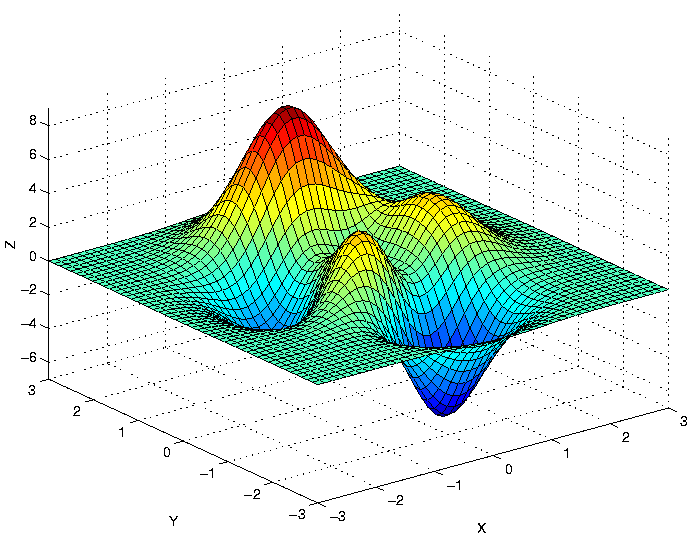
\includegraphics[width=0.8\textwidth, height=0.2\textheight]{chapter_3/files/peaks.png}
\caption{A function taking points in \(\mathbb{R}^2\) to
  \(\mathbb{R}\). Effectively, it can be thought of as a mathematical
  mountain range. [1]} 
\label{fig:circle}
\end{figure}
Upon visualizing this landscape, some natural questions arise such as
how the landscape is changing and how to quantify its salient
features. The gradient operates on the function \(f\) to produce a
vector field. It is this vector field that gives us insight into how
the underlying function is changing, and is defined as follows: 
\[
\nabla f = \sum_{i=1}^n \frac{\partial f}{\partial x_i} \hat{x_i}
\]
A few things to note here. First the gradient is defined for every
point \(x \in \mathbb{R}^n\). Additionally, the gradient tells you the
direction of steepest increase and points toward some other value on
the landscape \(f(x')\). Appropriately, when at a maxima or minima,
\(\nabla f = \vec{0}\) indicating that there is no distinct direction
of steepest ascent. 
\\\\
Of equal importance is studying the behavior of a vector field
\(\vec{V}\), and one way to do that is by taking a sum over how each
component is changing, which is realized as the divergence
operator. To accomplish this, we define the divergence operator as
follows: 
\[
\nabla  \cdot \vec{V} = \sum_{i=1}^n \frac{\partial V_{x_i}}{\partial
  x_i} \textnormal{ where \(V_{x_i}\) is the component in the
  \(\hat{x_i}\) direction} 
\]
The divergence quantifies flux density at a single point, and when
considering the net divergence in a region we can say whether or not
there is a source or a sink in the vector field. Note that implicitly
we need some notion of direction with regards to this flux density in
order to determine whether these is a source or a sink. Therefore, the
divergence is usually discussed with respect to an oriented
surface. All that this means is that moving forward we simply want
outward flux to be defined as positive, and influx to be negative. 
\\\\
You may have noticed that since the gradient spits out a vector field,
and the divergence eats a vector field and spits out a scalar, it may
be worthwhile to compose the two operations, and in fact it is! The
composition is known as the Laplacian and can be seen as a simple
summation of second derivatives: 
\[
\nabla \cdot \nabla f = \sum_{i=1}^n \frac{\partial^2 f}{\partial x_i^2}
\]
Beyond the math, the Laplacian is acting as an averaging operator,
telling us how a single point is behaving relative to its surrounding
points. As one may expect, this plays an important role in
establishing some sort of equilibrium. The Laplacian appears in
physics equations modeling diffusion, heat transport, and even
mass-spring systems. In the case of data science, once again the
Laplacian will lend us toward an equilibrium, this time with respect
to clustering. For our purposes, equilibrium will take the form of
partitions where data points are happily settled in their partition. 

\subsection{Calculus on Graphs}
Instead of concerning ourselves with functions on the real line, we
will now need to concern ourselves with functions on vertices and
functions on edges of simple, weighted graphs which we denote as
\(G(V,E)\) with an accompanying weight matrix \(W\). We specify the
set of vertices as \(V = \{1, 2, ... , n\}\), an edge going from
vertex \(i\) to vertex \(j\) as \(e = [i,j]\), and a weight matrix
\(W\) where \(w_{ij}\) corresponds to the weight of edge \(e =
      [i,j]\). With this notation in mind, we wish to define the two
      function spaces we will be working with: 
\begin{definition}[The Vector Space \(\mathbb{R}^V\)]
The space of real valued vertex functions \(f: V \rightarrow \mathbb{R}\).
\end{definition}
\begin{definition}[The Vector Space \(\mathbb{R}^E\)]
The space of real valued edge functions \(X: E \rightarrow
\mathbb{R}\) that are anti-symmetric such that \(X([i,j]) =
-X([j,i])\) 
\end{definition}
As we will see, \(\mathbb{R}^V\) will correspond to the manifold on
which we are performing the calculus while \(\mathbb{R}^E\)
corresponds to a vector field. Also note that the anti-symmetry of the
functions on \(\mathbb{R}^E\) corresponds to the sign of a vector in a
vector field. This is especially important in the formulation of a
gradient operator on a graph as we would like to capture steepest
ascent (going with the gradient) as well as steepest descent (going in
the exact opposite direction of the gradient). With this in mind, we
can now define the differential on a graph: 
\begin{definition}[Differential Operator on a Graph \(d\)]
The graph analogue of the gradient, a linear operator \(d:
\mathbb{R}^V \rightarrow \mathbb{R}^E\), defined as \(df([i, j]) =
f(j) - f(i)\). 
\end{definition}
This notion of a gradient should sit well with us. It looks quite
similar to our intro calculus version of a derivative except for
scaling and taking a limit. Furthermore, this is assigning a
derivative-like value to an edge, reinforcing our notion that
\(\mathbb{R}^E\) will be analogous to a vector field. 
\begin{exercise}[The Derivative on an Intuitive Graph]
Consider the Path Graph \(P_5\) with 5 vertices and 4 edges numbered
\(v_1...v_5\) and the vertex function \(f(v_i) = (3 - i)^2\). Draw the
graph and the function on top of the graph using a lollipop plot. From
there, calculate the differential about each vertex specifying the
orientation of the differential, and draw the differentials on the
graph. 
\end{exercise}
Now that we have one half of calculus generalized, let us look at the
other half of calculus: integration. Especially for those familiar
with quantum mechanics, the formulation of integration on a graph is
rather intuitive taking the form of an inner product. With this in
mind, we define two inner product spaces on functions of both edges
and vertices. 
\begin{definition}[Inner Product Space \((\mathbb{R}^V, \langle \cdot, \cdot \rangle_V)\)]
The space of real valued vertex functions equipped with an inner
product defined on functions such that \(\langle f, g \rangle_V =
\sum_{v \in V}f(v)g(v)\). 
\end{definition}
\begin{definition}[Inner Product Space \((\mathbb{R}^E, \langle \cdot, \cdot \rangle_E)\)]
The space of real valued edge functions equipped with an inner product
defined on functions such that \(\langle X, Y \rangle_E = \sum_{e \in
  E}w_e X(e)Y(e)\). 
\end{definition}
Note in both of these definitions, that in the limit of a very large
number of edges and vertices we return to standard notions of
integration as follows: 
\[
\langle f, g \rangle_V \leftrightarrow \int_{\mathbb{R}}f(x)g(x)dx
\]
\[
\langle X, Y \rangle_E \leftrightarrow \int_{\mathbb{R}^E}X(e)\cdot Y(e)d\mu_w
\]


\subsection{Local and Global Smoothness}
So far we have been building the machinery to understand the
Laplacian, and we are almost there. The big thing that we have been
working towards is actually a measure of global smoothness of vertex
functions on our graph. This is important to us as we will see that
"independently" smooth sections of the graph will correspond to
clusterings. To define smoothness, we actually consider the inner
product of the differentials of functions, corresponding to a measure
of total variation in the graph functions: 
\begin{definition}[Global Smoothness Measure \(\langle df, df \rangle_E\)]
Following the definitions thus far established, the global smoothness
is defined as: \[\langle df, df \rangle_E = \sum_{[i,j] \in E}w_e(f(j)
-f(i))^2\] 
\end{definition}
An important observation is that this function is trivially minimized
for constant functions. In other words, we have the following
implication for any function constant on \textit{all} vertices: 
\[
f(v) = c \rightarrow \langle df, df \rangle_E = 0
\]
This is important when we formulate the MinCut algorithm using this
measure of smoothness so to exclude the trivial (boring)
solution. However note that we wish to exclude a \textit{global}
constant solution. What would be very telling and indicate some
intimate relationship between vertices would be functions with compact
support that simultaneously force the global smoothness function to be
minimized. To be more concrete, can we find a set of indicator
functions defined on a partition of the vertices such that: 
\[
\langle d\mathbbm{1}_{v \in C_j}(v), d\mathbbm{1}_{v \in C_j}(v)
\rangle_E = 0 \: \: \: \forall \: \: \: C_j 
\]
\[
\sum_{j=1}^{|C|} \mathbbm{1}_{v \in C_j}(v) = \mathbf{1}
\]
From the definition of the differential, the existence of these vertex
functions would correspond to unique connected components in the
graph, with one indicator function per connected component. That is
great for us, as connected components make great clusters! However,
there is one final issue to wrap up before we can find these
functions. The global smoothness function is defined on the space
\((\mathbb{R}^E, \langle \cdot, \cdot \rangle_E)\), but we are looking
for functions in the space \((\mathbb{R}^V, \langle \cdot, \cdot
\rangle_V)\). Luckily, we can make this conversion, and finally
encounter the Laplacian.

\subsection{Existence of the Laplacian}
Before the Laplacian can finally be realized, we first need to
understand what an adjoint operator is: 
\begin{definition}[Adjoint Operator \(T^*\)] 
For any linear transformation \(T: V \rightarrow E\) between two
finite dimensional inner product spaces, there exists a unique map
\(T^*: E \rightarrow V\) such that for any elements \(v \in V\) and
\(e \in E\): 
\[
\langle v, T^*e \rangle_V = \langle Tv, e \rangle_E
\]
\end{definition}
Although this holds true for any two inner product spaces (regardless
of whether we are dealing with graphs), hopefully the notation in the
definition of the adjoint begins to offer a view into how it should be
used. For our operator \(d\), there exists an adjoint operator \(d^*\)
(called the \textit{co-differential}, corresponding to the divergence)
such that: 
\[
\langle df, df \rangle_E = \langle f, (d^*d)f \rangle_V
\]
\begin{definition}[The Discrete Divergence (Co-Diffferential) \(d^*\)]
To accompany the differential (gradient) we also have its adjoint
operator the co-differential, defined about a vertex \(i\) over an
edge function \(X([i, j])\) such that: \[d^*(X)(i) = \sum_{j \sim i
}w_{ij}X([i,j])\] 
\end{definition}
Now we are finally in the position to make some progress in finding
these functions representing clusters in the graph. From linear
algebra, we know that compositions of linear maps are linear maps and
that linear maps take the form of matrices. This allows us to call
this weird looking composition of operators the Laplacian and denote
it by the matrix \(L = (d^*d)\). Gluing the definition of the
co-differential together with the previous definition of the
differential, we can see that the composition of the co-derivative and
derivative takes the form of an operator acting on a vertex by summing
up the weights of the "derivatives" about that point. This new
operator is the Laplacian. 
\begin{definition}[The Graph Laplacian \(L\)]
The composition of operators \(L = d^*d\) acts upon a function in the
following way, adherent to the previously constructed definitions: \[ 
Lf = \sum_{j \sim i} w_{ij} (f(i) - f(j))\]
\end{definition}
From here, we note that from the definition of the dot product on the
space of vertex functions, the inner product reduces to our standard
notion of a dot product, resulting in a quadratic form. 

\[
\langle df, df \rangle_E = \langle f, Lf \rangle_V = f^TLf
\]

\section{Exploring the Graph Laplacian}
With the Graph Laplacian's existence confirmed and some insight into
its behavior from the continuous analogue, let us define in it in its
more computationally useful way: 
\[
L = D - W 
\]
Where \(D\) is a diagonal matrix with \(d_{ii} = \textnormal{deg}(i) =
\sum_{j \sim i} w_{ij}\) such that each weight is only counted once,
and W is the weight matrix previous defined. With this definition in
mind, the Laplacian simplifies as follows when acting on the vector
\(f\) where \(f(i)\) represents the \(i\)th coordinate: 
\[
(Lf)(i) = \sum_{j \sim i} f(i) w_{ij} - \sum_{j \sim i} f(j) w_{ij} =
\sum_{j \sim i} w_{ij}(f(i) - f(j)) 
\]
This summation goes to show that the Laplacian is acting as a
vertex-wise measure of local smoothness. Namely, how does the value at
a vertex relate to the values of its neighbors. An immediate
consequence is that for a given vertex \(i\), if \(f(i) = f(j)\) for
all neighbors \(j\), then the result of the Laplacian acting on that
vertex is 0. If the graph is fully connected, this tells us that the
constant function will minimize the above quadratic form. The same is
true for a disconnected graph as well, however, a disconnected graph
will have additional functions which minimize the quadratic form as
well, namely an indicator function for each connected
component. Therefore, finding the indicator functions on the
components is equivalent to finding a basis for the kernel of \(L\). 
\\\\
Mentioned in the very beginning, the continuous version of the
Laplacian told us how a point was behaving relative to its
neighbors. Massaging the above relation, one can see that the graph
Laplacian behaves analogously: 
\[
(Lf)(i) = d_{i} \bigg[ f(i) - \underbrace{\frac{1}{d_i} \sum_{j \sim
      i} w_{ij}f(j)}_\text{Average About \(i\)} \bigg] 
\]
With this in mind, the next thing to consider is how one would go
about finding these indicator functions corresponding to connected
components. Given that the Laplacian is symmetric, we can invoke the
Spectral Theorem to discover an orthonormal basis \(\{u_i\}\) for
\(L\) with corresponding eigenvalues \(\lambda_1 \leq \lambda_2 \leq
...\leq \lambda_n\). Since we are finding the kernel of \(L\), it
stands to reason that the indicator functions on the connected
components will be eigenvectors of \(L\) (really the eigenfunctions on
the vertices) corresponding to eigenvalues of 0. 
\begin{claim}[Spectrum of the Laplacian]
The multiplicity of \(\lambda = 0\) corresponds to the number of
connected components in the graph. Moreover, the associated
eigenvectors are mutually orthogonal and a linear superposition of
them can be found to form the constant function on the vertices. 
\end{claim}

\begin{exercise}[Fun with the Laplacian]
Consider a graph with weight matrix:
\[
W = 
\begin{bmatrix}
    0 & 0 & 1 & 0 & 3\\
    0 & 0 & 0 & 4 & 0\\
    1 & 0 & 0 & 0 & 2\\
    0 & 4 & 0 & 0 & 0\\
    3 & 0 & 2 & 0 & 0
\end{bmatrix}
\]
Draw the graph, then derive the Laplacian for this graph, showing your
work for calculating \(D\) as well. Confirm that any constant vector
resides in the kernel of \(L\). By inspection, MATLAB, or brute force
calculations, find the basis for the kernel of \(L\). Confirm that
these basis vectors are orthogonal. 
\end{exercise}
\begin{exercise}[Kernel of the Laplacian] Why is the Laplacian always
  Positive Semi-Definite? 
\end{exercise}
\begin{exercise}[Working with the Spectral Decomposition]
How would you find the number of nodes in a given connected component?
\end{exercise}

\section{Physical Examples}
\subsection{Simple Springs-Mass Systems}
Given that the Laplacian has a deep connection to physics, it makes
sense for us to explore this connection to gain some additional
understanding. The example which we will be exploring is a series of
mass-spring systems. Recall that there are two constituent equations
which we use to analyze spring-mass systems, given in below in
generalized coordinates (which is why they lack the equilibrium
length): 
\[
F = -kx
\]
\[
U = \frac{1}{2}kx^2
\]
Using generalized coordinates, we will attempt to understand how the
Laplacian gives rise to solutions which are in equilibrium, starting
with a simple 3-mass, 3-spring system, with all masses equal, but
potentially different spring constants. Now, we need to pose this as a
function on a graph. To analyze this system, we shall think about the
vertex function representing the position of a particular mass, with
springs represented by weights along edges. As one might expect, by
formulating the Laplacian for this system we can then find a
configuration that minimizes internal forces and therefore energy; in
other words, a mechanical equilibrium. 
\begin{figure}[ht]
\centering
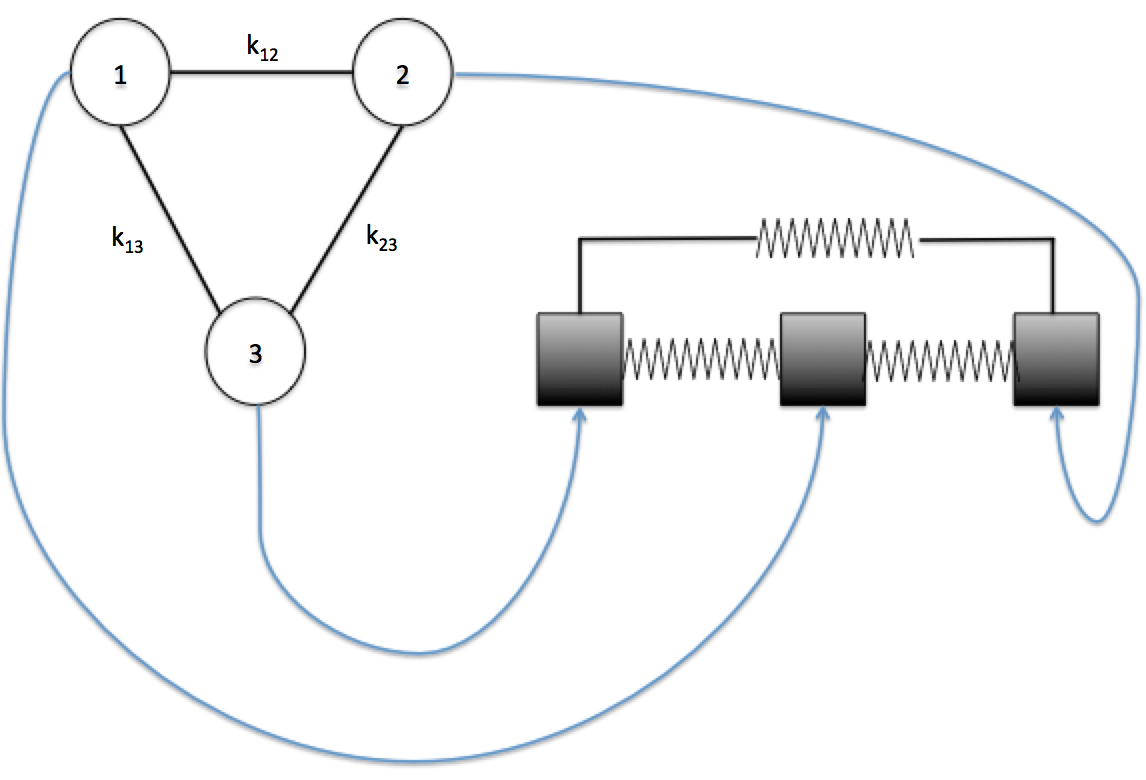
\includegraphics[width=0.8\textwidth, height=0.4\textheight]{chapter_3/files/springs.png}
\caption{Showing the translation between a simple graph and a physical
  problem. Note that the vertex function corresponds to the position
  of the masses!} 
\label{fig:springs}
\end{figure}

For a general configuration as shown in Figure 2, we can formulate the
Laplacian as one would expect.
\[
L = \underbrace{\begin{bmatrix}
    k_{12} + k_{13} & 0 & 0 \\
    0 & k_{12} + k_{23}   & 0 \\
    0 & 0 & k_{13} + k_{23} 
\end{bmatrix}}_\text{\(D\)} -
\underbrace{
\begin{bmatrix}
    0      & k_{12} & k_{13} \\
    k_{12} & 0      & k_{23} \\
    k_{13} & k_{23} & 0 
\end{bmatrix}}_\text{\(W\)}
\]
\[
L = \begin{bmatrix}
    k_{12} + k_{13} & -k_{12} & -k_{13} \\
    -k_{12} & k_{12} + k_{23} & -k_{23} \\
    -k_{13} & -k_{23} & k_{13} + k_{23} 
\end{bmatrix}
\]
By inspection we can confirm that any constant vector will be in the
kernel of the Laplacian! Beyond the math, this says that if we shift
our axes, physics will still work in the exact same way. From here,
lets explore the Laplacian a bit more by having it act on a position
vector: 
\[
Lf = \begin{bmatrix}
    k_{12} + k_{13} & -k_{12} & -k_{13} \\
    -k_{12} & k_{12} + k_{23} & -k_{23} \\
    -k_{13} & -k_{23} & k_{13} + k_{23} 
\end{bmatrix}
\begin{bmatrix}
x_1 \\
x_2\\
x_3
\end{bmatrix}
\]
Working out the result for the first coordinate, we see the following: 
\[
(Lf)_1 = 
    (k_{12} + k_{13})x_1 -k_{12}x_2 -k_{13}x_3 
\]
\[
(Lf)_1 = 
    k_{12}(x_1 - x_2) + k_{13}(x_1 - x_2) = \sum_{j \sim i} k_{1j}(x_1 - x_j)
\]
Or more generally, for any coordinate we can see that we get back the
behavior we expect: 
\[
(Lf)_i = \sum_{j \sim i} k_{ij}(x_i - x_j)
\]
If we very suggestively negate the matrix product, we can see that
Hooke's law stems from the Laplacian! With defined initial conditions,
one could use this to simulate the  time evolution of the system. 
\[
F = -Lf
\]
For equilibrium, it follows from Newton's Laws that the total force
acting on any mass must be zero, therefore at equilibrium the
following condition must hold: 
\[
-Lf = 0
\]
Any function \(f\) which satisfies the above equation is known as a
\textit{harmonic}, with the above equation for equilibrium being known
as \textit{Laplace's Equation}. The next thing to consider is how does
one obtain a formulation of the potential energy in the system? By
observing that the potential energy for the whole system is
proportional to the sum of the displacements squared, we can see how
the Laplacian also relates to the potential energy: 
\[
U_{sys} = \frac{1}{2} \sum_{[i,j] \in E} k_{ij} \big[ x_i - x_j\big]^2
= \frac{1}{2} \sum_{[i,j] \in E} k_{ij} \big[ f(i) - f(j)\big]^2 
\]
From here, we can note that this shows that the total potential energy
takes the form of the global smoothness measure, meaning that a
minimization of energy corresponds to having the smoothest
functions. We can see that the following holds, with this quantity in
harmonic analysis being known as the \textit{Dirichlet energy} of the
system in harmonic analysis: 
\[
U_{sys} = \frac{1}{2} \langle df, df \rangle_E = \frac{1}{2} \langle f, Lf \rangle_V
\]
\subsection{Simple Spring-Mass Systems: A Second Perspective}
For a different perspective, consider a slightly different expansion
of the Laplacian acting on the position function:  
\[
Lf = \begin{bmatrix}
    k_{12} + k_{13} & -k_{12} & -k_{13} \\
    -k_{12} & k_{12} + k_{23} & -k_{23} \\
    -k_{13} & -k_{23} & k_{13} + k_{23} 
\end{bmatrix}
\begin{bmatrix}
x_1 \\
x_2\\
x_3
\end{bmatrix}
\]
\[
(Lf)_1 = 
    (k_{12} + k_{13})x_1 -k_{12}x_2 -k_{13}x_3 
\]
\[
(Lf)_1 = 
    (k_{12} + k_{13}) \bigg[ x_1 - \frac{k_{12}}{k_{12} + k_{13}} x_2
  - \frac{k_{13}}{k_{12} + k_{13}} x_3 \bigg] 
\]
\[
(Lf)_1 = 
    \textnormal{deg}(x_1) \bigg[ x_1 - \frac{1}{\textnormal{deg}(x_1)}
      \sum_{j \sim i} k_{1j}x_j  \bigg] 
\]
Or, by symmetry, more generally:
\[
(Lf)_i = 
    \textnormal{deg}(x_i) \bigg[ x_i - \frac{1}{\textnormal{deg}(x_i)}
      \sum_{j \sim i} k_{ij}x_j  \bigg] 
\]

This is telling us that the Laplacian acting on the vertex function
(vector of mass positions) spits out how different that particular
mass's position is relative to the weighted average of its
neighbors. Note that the weight comes from the relative spring
constants, and that the entire thing is scaled by the sum of all of
the springs connected to that note. In a sense this is telling us that
stronger springs and very well connected masses will tend to be what
determines a minimal energy configuration. It also says that if we
disturb the system from equilibrium, we will be most unhappy if we
touch the most important masses. Moreover, that as the system evolves
over time the system will tend toward an equilibrium where the
position of a certain mass equals the weighted average of it's
neighbor's positions.

\subsection{Complex Spring-Mass Systems and Data Science}
Consider a gigantic mess of springs and masses intertwined: what the
Laplacian has to say about its behavior? Well quite a lot, but at the
high level, it can normally tell us how feasible it is to untangle the
blob into separate systems. If we could find two completely decoupled
systems, it would be completely analogous to finding two disconnected
components in the graph. The constant offset in the coordinates along
a connected component does not change the energy of the system, only
where the entire system resides in space. Likewise, if we can move
some entire subset of the masses somewhere else, and not change the
energy of the system, it stands to reason that those masses form an
isolated system.  
\\\\
Despite our best efforts in trying to untangle a mess of masses and
springs, we may not always be able to always separate the
nightmare. That being said, we can \textit{always} find a
configuration which minimizes the energy of the spring mass
system. With some insight from the Laplacian, we can see that to
minimize the internal forces (and therefore the energy), we will want
to keep the large spring constants and the well connected masses in
equilibrium, and if we have to perturb some part of the system, we
will preferentially stretch or compress the weaker springs and less
important masses. With this insight in hand, we can make a leap back
to data science. 
\\\\
Consider a data set where you have data points, and some measure of
similarity between the data points. The data points are analogous to
the masses, and the similarity analogous to spring constants. Should
you have data points with lots of very close neighbors, you do not
want to pull them apart: it makes no sense as you would be disturbing
that cluster's natural equilibrium. That being said, on the fringes of
clusters we may expect some weak similarity with data not actually in
the cluster, and certainly fewer relationships. As such if we want to
minimize the energy of the system, we will want to keep the tightly
packed parts of the clusters close together, at the expense of
disturbing a few of the outliers. When at a minimal energy
configuration, we should have a nice partitioning into quasi-isolated
systems which very nearly behave independently. With this in mind, all
that remains is finally making a decision on the minimal energy
configuration, and making an appropriate delineation of what we
consider to be the isolated isolated systems corresponding to
clusters.  

\section{Approximating MinCut}
In order to finally use the Laplacian for clustering, consider the
MinCut Algorithm: 
\\\\
\noindent
\textbf{Input:} A Graph \(G(V, E, W)\)
\\\\
\noindent
\textbf{Output:} Two sets \(A\) and \(B\) such that \(G = A \coprod
B\) such that the cut is minimized: 
\[
\textnormal{min cut}(A,B) = \frac{\sum_{i \in A, j\in B}
  w_{ij}}{\textnormal{min} \{|A|, |B|\} } 
\]
Returning to the analogy of springs and masses, this objective
function is trying to separate the system such that the fewest and
weakest springs separate the clusters while maximizing the cluster
size. This prevents us from making a trivial cut (one of the sets
being empty) and generally forces the two clusters to be of
approximately the same size. From here, we note that if the graph
functions with which we are dealing are of the form \(f: V \rightarrow
\{0,1\}\), we can suggestively rewrite the the numerator of the cut
objective function, and note it corresponds to the global smoothness! 
\[
\textnormal{min cut}(A,B) = \frac{\sum_{i \in A, j\in B} w_{ij} (f(i)
  - f(j))^2}{\textnormal{min} \{|A|, |B|\} } 
\]
\[
\textnormal{min cut}(A,B) = \frac{f^TLf}{\textnormal{min} \{|A|, |B|\} }
\]
From here we can note that the \(\textnormal{min} \{|A|, |B|\}\) under
the assumed functional form is simply counting the number of 1's in
the vector, then we can see that the objective function is really just
a Rayleigh quotient! 
\[
\textnormal{min cut}(A,B) = \frac{f^TLf}{f^Tf }
\]
Now, we need to perform this minimization, while excluding the obvious
all 1's solution. To do this, we simply impose the constraint that the
solution must be orthogonal to the constant solution, invoke formulate
Rayleigh's theorem which is at the core of computing these clusters. 
\begin{theorem}[Rayleigh's Theorem]
The following quotient is minimized when \(f = u_2\), the eigenvector
corresponding to \(\lambda_2\): 
\[
\textnormal{arg min}_{f \perp \mathbf{1}} = \frac{f^TLf}{f^Tf }
\]
\end{theorem}

From here, we note that given the spectral decomposition of the
Laplacian, that the minimal value is obtained when \(f = u_2\), or the
eigenvector of the Laplacian corresponding to \(\lambda_2\) for any
graph. Note that for a graph with one connected component, this
constraint excludes a bad answer to the problem. This effectively
imposes that the first eigenvector, which is always in the kernel of
\(L\) since every graph has at least one connected component, cannot
minimize the quantity. However, this DOES NOT exclude a good answer in
the case of a disconnected graph as subsequent eigenvalues will have
value 0 and allow for the minimization to be obtained.  In practice,
this will seldom be the case, and usually \(\lambda_2 > 0\), so we get
an imperfect cut. The result is an eigenvector which is not a perfect
indicator function, but can be subsequently used for clustering. Due
to \textit{Cheeger's Inequality}, the second eigenvalue is related to
a property of the graph known as the conductance, which more or less
says how meaty the MinCut was: a lower conductance implies a better
MinCut. 

If you wish to find k-clusters, simply look at the bottom \(k\)
eigenvalues (excluding \(\lambda_1 = 0\)), and use the associated
eigenvectors as a basis for new data points to perform
clustering. These basis vectors will be mutually orthogonal as
guaranteed by the spectral theorem, and allow for a representation of
any new data points encountered. To cluster a new datapoint, simply
consider its representation in the new basis, and perform regular
k-means clustering. An intuitive depiction of the spectral clustering
and the resultant eigenvectors is shown in Figure 3, highlighting that
these vectors should be orthogonal and ideally be very sharp
indicators of partition membership. Of course this is subject to
appropriate graph preprocessing. 
\begin{figure}[ht]
\centering
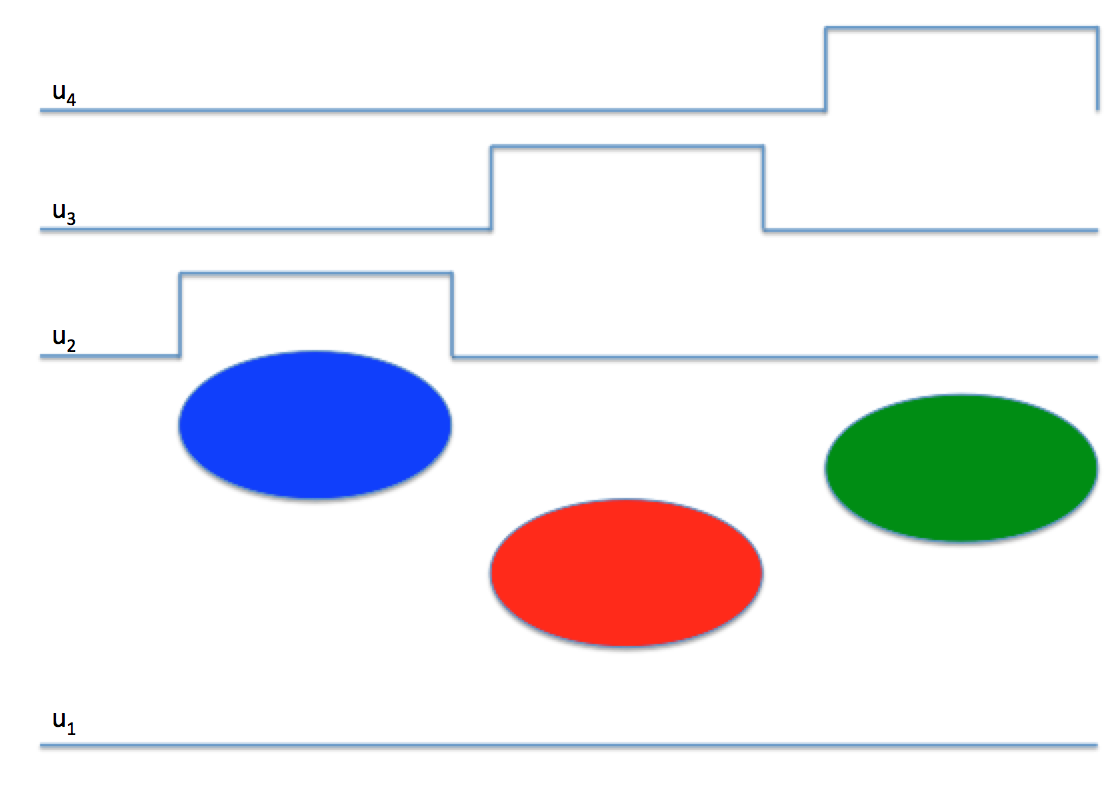
\includegraphics[width=0.8\textwidth, height=0.3\textheight]{chapter_3/files/cluster.png}
\caption{Intuitive depiction of eigenvectors minimizing the Rayleigh
  Quotient. Note their indicator behavior and mutual orthogonality. In
  the real world, they will be less sharp and more squiggly.} 
\label{fig:circle}
\end{figure}
\section{Closing Remarks}
Wrapping up this lecture, we close with some summarizing
remarks. Namely, the big picture of spectral clustering, summarized in
four steps: 
\begin{enumerate} 
\item Construct a weight matrix \(W\) for the dataset you wish to
  cluster. A common method of defining similarity is \(w_{ij} =
  \exp({||x_i - x_j||^2 / \sigma^2})\). 
\item Construct the induced Laplacian \(L = D-W\).
\item Find the eigendecomposition of \(L\) and select the number of
  basis vectors according to the number of clusters you expect. 
\item Run k-means in the new basis.
\end{enumerate}

\section{Some More for the Advanced Reader}
There were a few more tidbits mentioned in class, which should be
noted here, but are not directly applicable to the homework. One
particularly interesting piece was on the PseudoInverse of the
Laplacian. You may remember that the Laplacian took us from position
to force. Well, the PseudoInverse does the opposite giving us the
position from a set of forces. Therefore, the PseudoInverse of the
Laplacian induces a distance kernel. The example mentioned in class
was about the Euclidean average commute time distance, namely
\(\langle x, L^{-1}x \rangle\) which sort of tells you how bad your
commute will be going to and from a certain area of the graph.  
\\\\
One other very cool point from class was that the eigendecomposition
is not a convex problem, but we still do it all the time! While convex
problems are inherently easy, non-convex does not imply impossible or
even that difficult. The take-away being that just because a problem
is non-convex does not mean it's the end of the world :) 

